% \iffalse
%<*gobble>
% $Id: rviewport.dtx,v 1.2 2011-08-27 22:53:32 boris Exp $
%
% Copyright 2011, Boris Veytsman <borisv@lk.net>
% This work may be distributed and/or modified under the
% conditions of the LaTeX Project Public License, either
% version 1.3 of this license or (at your option) any 
% later version.
% The latest version of the license is in
%    http://www.latex-project.org/lppl.txt
% and version 1.3 or later is part of all distributions of
% LaTeX version 2003/06/01 or later.
%
% This work has the LPPL maintenance status `maintained'.
%
% The Current Maintainer of this work is Boris Veytsman
%
% This work consists of the file rviewport.dtx and the
% derived files rviewport.sty, rviewport.dtx. 
%
% \fi 
% \CheckSum{110}
%
%
%% \CharacterTable
%%  {Upper-case    \A\B\C\D\E\F\G\H\I\J\K\L\M\N\O\P\Q\R\S\T\U\V\W\X\Y\Z
%%   Lower-case    \a\b\c\d\e\f\g\h\i\j\k\l\m\n\o\p\q\r\s\t\u\v\w\x\y\z
%%   Digits        \0\1\2\3\4\5\6\7\8\9
%%   Exclamation   \!     Double quote  \"     Hash (number) \#
%%   Dollar        \$     Percent       \%     Ampersand     \&
%%   Acute accent  \'     Left paren    \(     Right paren   \)
%%   Asterisk      \*     Plus          \+     Comma         \,
%%   Minus         \-     Point         \.     Solidus       \/
%%   Colon         \:     Semicolon     \;     Less than     \<
%%   Equals        \=     Greater than  \>     Question mark \?
%%   Commercial at \@     Left bracket  \[     Backslash     \\
%%   Right bracket \]     Circumflex    \^     Underscore    \_
%%   Grave accent  \`     Left brace    \{     Vertical bar  \|
%%   Right brace   \}     Tilde         \~} 
%
%\iffalse
%    \begin{macrocode}
\documentclass{ltxdoc}
\usepackage{array,graphicx}
\usepackage{url,amsmath,hypdoc}
\usepackage{rviewport}
\newcommand\progname[1]{\textsl{#1}}
\DoNotIndex{\NeedsTeXFormat, \ProvidesPackage, \def, \hspace}
\DoNotIndex{\futurelet, \@gobble, \ifx, \else, \fi, \relax}
\DoNotIndex{\ifmmode, \fi, \allowbreak}
\PageIndex
\CodelineIndex
\RecordChanges
\EnableCrossrefs
\begin{document}
  \DocInput{rviewport.dtx}
\end{document}
%    \end{macrocode}
%</gobble> 
% \fi
% \MakeShortVerb{|}
%
%\GetFileInfo{rviewport.sty}
% \title{Relative Viewport for Graphics Inclusion\thanks{\copyright
% Boris Veytsman, 2011. E-mail: \texttt{borisv@lk.net}}}
% \author{Boris Veytsman\thanks{This work was partially supported by
% The Food and Agriculture Organization of the United Nations}}
% \date{\filedate, \fileversion}
% \maketitle
%
% \begin{abstract}
%   The package adds a new keyword |rviewport| to the
%   \progname{graphicx} package specifiying Relative Viewport for
%   graphics inclusion: a window defined by the given fractions of the
%   natural width and height of the image.
% \end{abstract}
%
% \tableofcontents
%
% \clearpage
%
%\section{User Interface}
%\label{sec:interface}
%
% Package \progname{graphicx} provides a useful keyword |viewport|
% which allows to show just a part of an image.  However, one needs to
% put there the actual coordinates of the viewport window.  Sometimes
% it is useful to have relative coordinates as fractions of
% natural size.  For example, one may want to print a large image on a
% spread, putting a half on a verso page, and another half on the next
% recto page.  For this one would need a viewport occupying exactly
% one half of the file's bounding box, whatever the actual width of the
% image may be. 
%
% Here we define the new option |rviewport| for
% Relative Viewport.  It works like this.  Suppose the image has the
% bounding box $x_{ll}$, $y_{ll}$, $x_{ur}$, $y_{ur}$.  We give four
% numbers $\xi_{ll}$, $\eta_{ll}$, $\xi_{ur}$, $\eta_{ur}$, and the viewport
% coordinates become
% \begin{align*}
%   x'_{ll} &= x_{ll} + \xi_{ll}\Delta_x\\
%   y'_{ll} &= y_{ll} + \eta_{ll}\Delta_y\\
%   x'_{ur} &= x_{ll} + \xi_{ur}\Delta_x\\
%   y'_{ur} &= y_{ll} + \eta_{ur}\Delta_y
% \end{align*}
% where
% \begin{align*}
%   \Delta_x &= x_{ur} - x_{ll}\\
%   \Delta_y &= y_{ur} - y_{ll}
% \end{align*}
% This means that the left half of the image can be defined as
% |rviewport = 0 0 0.5 1|, 
% and the right half can be defined as  |rviewport = 0.5 0 1 1|.
% 
% The package may be loaded before or after \progname{graphicx}
% package.  
%
%
%\section{Examples}
%\label{sec:examples}
%
%
% \def\Example#1{%
%   \begin{center}
%     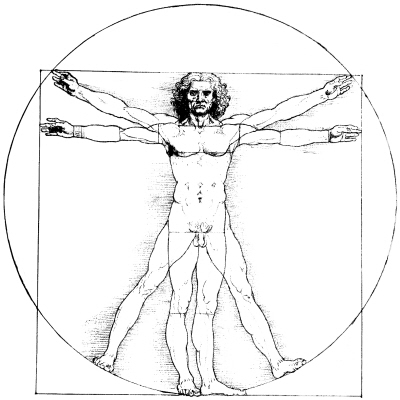
\includegraphics[rviewport=#1,clip]{vitruvian}\\*
%     \cmd{\includegraphics}[rviewport=#1,clip]\texttt{\{vitruvian\}}
%   \end{center}}
%   
% \Example{0 0 1 1}
% \Example{0 0 0.5 1}
% \Example{0.5 0 1 1}
% \Example{0 0 0.5 0.5}
% \Example{0 0.5 1 1}
% \Example{0 0 1 0.5}
% \Example{0.4 0.6 0.6 0.9}
%
%
%\StopEventually{}
%
% \clearpage
% 
% \section{Implementation}
% \label{sec:implementation}
% 
%
%\subsection{Declarations}
%\label{sec:decl}
% 
%  We start with declaration, who we are:
%
%
%    \begin{macrocode}
%<*style>
\NeedsTeXFormat{LaTeX2e}
\ProvidesPackage{rviewport}
[2011/08/27 v1.0 Relative viewport for graphics inclusion]
%    \end{macrocode}
%
% The package \progname{graphicx} loads \progname{keyval}, but in case
% we are loaded before \progname{graphicx} we require it here:
%    \begin{macrocode}
\RequirePackage{keyval}
%    \end{macrocode}
% 
%
%\subsection{The New Key}
%\label{sec:key}
%
% We add a new key for the \progname{graphicx} package: 
%    \begin{macrocode}
\define@key{Gin}{rviewport}
           {\let\Gin@viewport@code\Gin@rviewport\Gread@parse@rvp#1 \\}
%    \end{macrocode}
%
%
% \begin{macro}{\Gread@parse@rvp}
%   We parse four numbers into the corresponding macros:
%    \begin{macrocode}
\def\Gread@parse@rvp#1 #2 #3 #4 #5\\{%
  \def\Gin@vllx{#1}%
  \def\Gin@vlly{#2}%
  \def\Gin@vurx{#3}%
  \def\Gin@vury{#4}}%
%    \end{macrocode}
%   
% \end{macro}
%
% \begin{macro}{\Gin@rviewport}
%   And the viewport code.  Note that |pdftex.def| relies on
%   the values of |\Gin@v...| macros, so we redefine them as well. 
%    \begin{macrocode}
\def\Gin@rviewport{%
  \let\Gin@ollx\Gin@llx
  \let\Gin@olly\Gin@lly
  \let\Gin@ourx\Gin@urx
  \let\Gin@oury\Gin@ury
  \Gin@nat@width\Gin@urx\p@
  \advance\Gin@nat@width-\Gin@llx\p@
  \Gin@nat@height\Gin@ury\p@
  \advance\Gin@nat@height-\Gin@lly\p@
  \dimen@\Gin@vurx\Gin@nat@width
                      \edef\Gin@vurx{\strip@pt\dimen@}%
  \advance\dimen@\Gin@llx\p@
                      \edef\Gin@urx{\strip@pt\dimen@}%
  \dimen@\Gin@vury\Gin@nat@height
                      \edef\Gin@vury{\strip@pt\dimen@}%
  \advance\dimen@\Gin@lly\p@
                      \edef\Gin@ury{\strip@pt\dimen@}%
  \dimen@\Gin@vllx\Gin@nat@width
                      \edef\Gin@vllx{\strip@pt\dimen@}%
  \advance\dimen@\Gin@llx\p@
                    \edef\Gin@llx{\strip@pt\dimen@}%
  \dimen@\Gin@vlly\Gin@nat@height
                      \edef\Gin@vlly{\strip@pt\dimen@}%
  \advance\dimen@\Gin@lly\p@
                     \edef\Gin@lly{\strip@pt\dimen@}}
%    \end{macrocode}
%   
% \end{macro}
%
%
%
%\subsection{The Last Words}
%\label{sec:last}
%
%
%
%    \begin{macrocode}
%</style>
%    \end{macrocode}
%\Finale
%\clearpage
%
%\PrintChanges
%\clearpage
%\PrintIndex
%
\endinput
